%=========================================================
\chapter{Modelo del Alcance}
\label{cap:reqUsr}

En este capítulo se modela el alcance del sistema. Se presentan inicialmente los Actores involucrados y sus requerimientos, especificando cuales se alcanzaron en la primera iteración y cuales serán trabajados en la segunda iteración. Después se presentan los requerimientos funcionales de esta iteración y al final se presenta el modelo Físico y Lógico del sistema.


%---------------------------------------------------------
\section{Modelado de Usuarios}
\cdtInstrucciones{
	Identifique los actores que estarán involucrados en los procesos relacionados con el sistema para esta iteración de desarrollo. Ponga énfasis en los procesos involucrados.
}

\subsection{Organigrama de la Empresa}



\begin{figure}[htbp]
	\begin{center}
		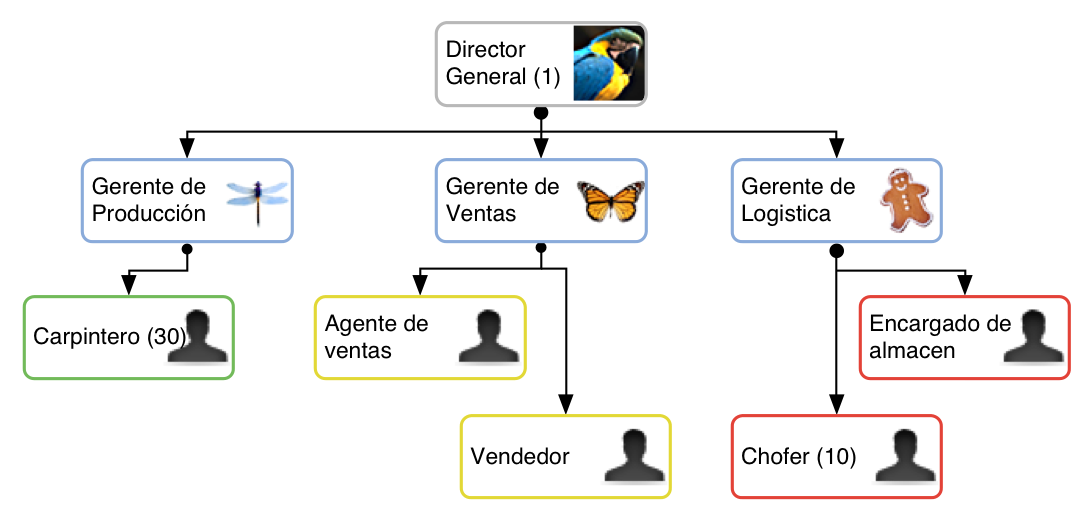
\includegraphics[width=.8\textwidth]{images/organigramaEm}
		\caption{Organigrama de la Mueblería Quetzal S. A. de C. V.}
		\label{fig:organigrama}
	\end{center}
\end{figure}


%---------------------------------------------------------
\begin{Usuario}{\subsection{Gerente de Ventas}}{
		Es el encargado de todas las operaciones de ventas al mayoreo y al menudeo. coordina y supervisa el trabajo de los Agentes de Ventas y Encargados de Tienda.
		Reporta directamente al Gerente de Operaciones
	}
	\item[Responsabilidades:] \cdtEmpty
	\begin{itemize}
		\item Supervisar la operación de ventas.
		\item Plantear y supervisar el logro de las metas de ventas de la empresa y su crecimiento económico.
		\item ...
	\end{itemize}

	\item[Perfil:] \cdtEmpty
	\begin{itemize}
		\item Amplia experiencia en el ramo.
		\item Licenciatura como mínimo.
		\item ...
	\end{itemize}
	\item[Procesos en los que participa:] \cdtEmpty
	\begin{itemize}
		\item PC-V01 Aprobar las órdenes de compra al mayoreo.
		\item PC-V02 Supervisar las ventas al menudeo.
		\item PC-V03 Elaborar informe de ventas mensual.
		\item ...
	\end{itemize}
\end{Usuario}

%---------------------------------------------------------
\begin{Usuario}{\subsection{Agente de Ventas}}{
		...
	}
	\item[Responsabilidades:] \cdtEmpty
	\begin{itemize}
		\item ...
	\end{itemize}

	\item[Perfil:] \cdtEmpty
	\begin{itemize}
		\item ...
	\end{itemize}
	\item[Procesos en los que participa:] \cdtEmpty
	\begin{itemize}
		\item PC-V08 Venta al Mayoreo.
		\item ...
	\end{itemize}
\end{Usuario}


%---------------------------------------------------------
\section{Requerimientos de usuario}

\cdtInstrucciones{
	Identifique y describa los requerimientos funcionales del sistema señalando: id, nombre, descripción y Pendiente.
}

\begin{table}[htbp!]
	\begin{requerimientosU}
		%Eidan
		\FRitem{RU1}{Ver reportes}{Se necesita generar y visualizar los reportes sobre comidas, baños del infante}{2}{\TODO}
		\FRitem{RU2}{Ver antecedentes médicos}{Debe de ser posible visualizar los antecedentes médicos del infante}{4}{\TODO}
		\FRitem{RU3}{Ver historial médico reciente}{Se necesita ver las atenciones médicas recientes del infante}{4}{\TODO}
		\FRitem{RU4}{Ver salón infante}{Se requiere que los profesores y padres conozcan en qué salón está cada infante.}{2}{\TODO}
		\FRitem{RU5}{Hacer menú alternativo}{Los infantes tendrán menús diferentes según su edad}{3}{\TODO}
		\FRitem{RU6}{Ver menú alternativo}{Los menús alternativos deben de ser visibles por los tutores de los infantes}{3}{\TODO}
		\FRitem{RU7}{Maestros por grupo}{Se necesita conocer quienes están a cargo de cada grupo}{2}{\TODO}
		\FRitem{RU8}{Registro ingesta}{Se requiere poder registrar qué cantidad de comida comió cada infante en una hora de comida.}{2}{\TODO}
		\FRitem{RU9}{Registro evacuación}{Se requiere poder registrar cuándo y qué tipo de evacuaciones tuvo un infante después de que las tenga.}{2}{\TODO}
		%ya 
		%BEGIN PARTE ANGEL
		\FRitem{RU10}{Registro de observaciones individuales}{La maestra necesita poder registrar observaciones de un infante individualmente.}{1}{\TODO}
		\FRitem{RU11}{Registro de pertenencias}{Es necesario tener un registro de las pertenencias de cada infante.}{1}{\TODO}
		\FRitem{RU12}{Crear menú mensual}{La nutrióloga debe de poder generar un menú de comidas para el mes.}{3}{\TODO}
		\FRitem{RU13}{Crear menú alternativo}{Se requiere poder generar un menú alternativo para infantes que lo requieran.}{3}{\TODO}
		\FRitem{RU14}{Registro atención médica}{Se quiere poder registrar la atención que fue recibida por un infante después de ser atendido por el médico.}{4}{\TODO}
		\FRitem{RU15}{Registro de desempeño}{Los profesores deben de poder registrar el desempeño en las actividades de los infantes.}{5}{\TODO}
		\FRitem{RU16}{Registro tareas y recados}{Los profesores deben de poder gestionar un registro de tareas y recados.}{5}{\TODO}
		\FRitem{RU17}{Registro días inhábiles}{El secretario registra los días inhábiles en el calendario.}{3}{\TODO}
		\FRitem{RU18}{Restricción de privilegios}{Sistema de privilegios: Se necesita limitar a las personas para que no todos tengan control sobre la guardería.}{1}{\TODO}
		%END PARTE ANGEL
		%BEGIN PART JOSUE
		\FRitem{RU19}{Registro de datos}{Es necesario tener datos personales de los tutores y del personal de la guardería.}{1}{\TODO}
		\FRitem{RU20}{Plan de estudios}{Se precisa conocer el plan de estudios activo.}{3}{\TODO}
		\FRitem{RU21}{Control de entradas y salidas}{Se busca tener un control de salidas y entradas del infante}{2}{\TODO}
		\FRitem{RU22}{Expediente médico}{Es necesario tener un expediente por infante que contenga sus datos básicos.}{4}{\TODO}
		\FRitem{RU23}{Cuidados especiales}{La maestra necesita saber si un niño requiere cuidados especiales por alguna situación de salud.}{4}{\TODO}
		\FRitem{RU24}{Consulta de horas de comida}{Los tutores deben de poder conocer los horarios de comidas de los infantes.}{2}{\TODO}
		\FRitem{RU25}{Selección de información según el hijo}{Un tutor necesita poder acceder a la información de todos sus hijos}{1}{\TODO}
		
	\end{requerimientosU}
	\caption{Requerimientos funcionales del sistema.}
	{\footnotesize\em Para leer correctamente esta tabla vea la leyenda en la Tabla~\ref{tbl:leyendaRF} en la página~\pageref{tbl:leyendaRF}.}
	\label{tbl:reqFunc}
\end{table}

\begin{table}[htbp!]
	\begin{requerimientosU}
		% <- Lo dejé hasta aquí
		\FRitem{RU26}{Visualización de hijos por profesor}{Cada profesor debe poder acceder a la información de los infantes que tiene a su cargo}{1}{\TODO}
		\FRitem{RU27}{Registro de actividades grupales}{Es necesario contar con un registro de actividades por grupo.}{1}{\TODO}
		%END PART JOSUE
		\FRitem{RU28}{Revisión de Actividades}{Los tutores deben de poder revisar las  actividades que sus hijos tienen asignadas.}{1}{\DONE}
		\FRitem{RU29}{Notificaciones de emergencia}{Son requeridas formas de notificar a los tutores situaciones de emergencia relacionadas con sus hijos.}{5}{\TODO}
		\FRitem{RU30}{Entrega de avisos}{Debe de haber una forma de entregar avisos a los tutores.}{5}{\DONE}
		\FRitem{RU31}{Calenadrizar eventos}{Se quiere un calendario de eventos mensuales para que la comunidad escolar se mantenga informada de las actividades que requieran especial atención de los tutores.}{3}{\DOING}
		\FRitem{RU32}{Evacuaciones Sospechosas}{Cuando un infante haya tenido múltiples evacuaciones sospechosas en un periodo corto de tiempo, se le debe de notificar a su tutor.}{5}{...}
		\FRitem{RU33}{Días Inhábiles}{Los tutores pueden ver los días inhábiles}{1}{\DONE}
		\FRitem{RU34}{Consulta de dudas}{Los tutores deben de tener una forma de consultar dudas con los docentes.}{5}{\TODO}
		\FRitem{RU35}{Registro de Salas}{Deben de poder registrarse salas y asignarles un tipo.}{1}{\DONE}
	\end{requerimientosU}
	\caption{Requerimientos funcionales del sistema.}
	{\footnotesize\em Para leer correctamente esta tabla vea la leyenda en la Tabla~\ref{tbl:leyendaRF} en la página~\pageref{tbl:leyendaRF}.}
	\label{tbl:reqFunc}
\end{table}


%---------------------------------------------------------
\section{Especificación de plataforma}

\cdtInstrucciones{
	Coloque un diagrama y su descripción para aclarar el tipo de solución propuesta. \\

	En esta sección se debe aclarar:

	\begin{description}
		\item[Tipo de sistema:] Web, aplicación móvil, de escritorio, híbrida, etc.
		\item[Software requerido:] Programas que se deberán instalar, desde el sistema operativo, compiladores, interpretes, servidores, etc.
		\item[Hardware requerido:] CPU, núcleos, velocidad, memoria, disco duro, etc.
		\item[servicios:] De conexión, seguridad, firewall, respaldo de energía, redundancia, uso de raids, etc.
	\end{description}
}

\begin{figure}[htbp!]
	\begin{center}
		\fbox{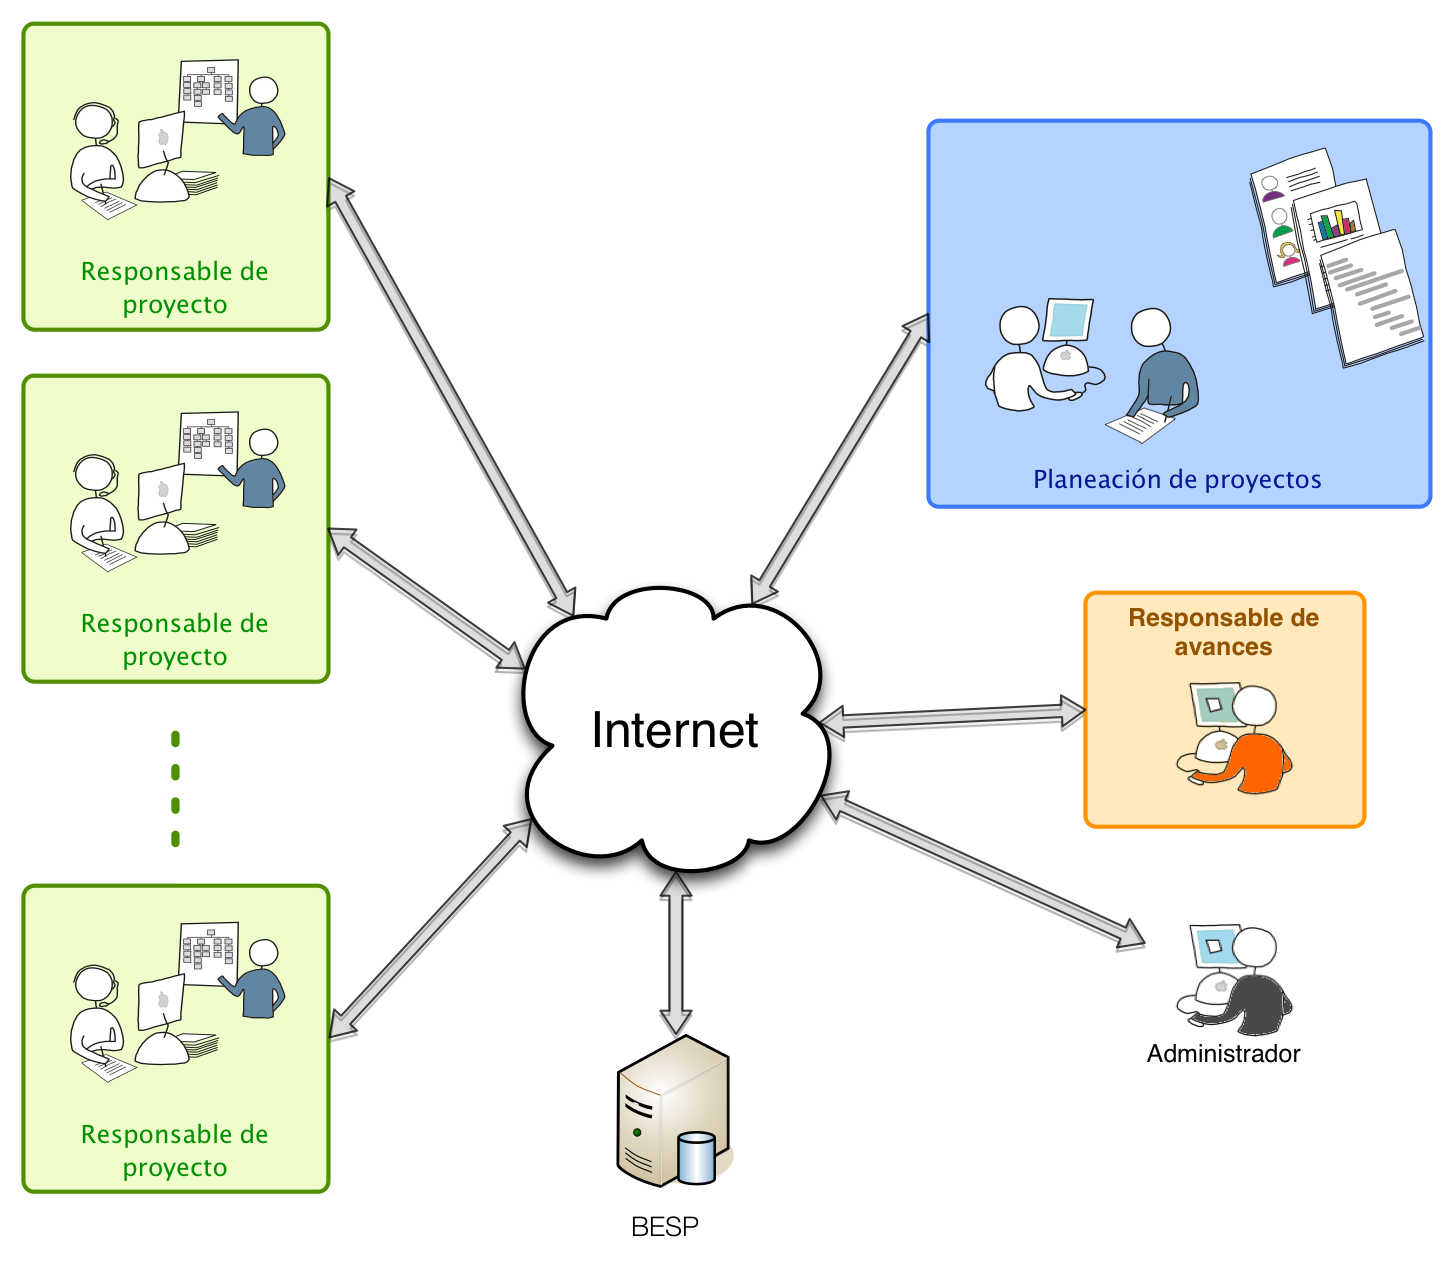
\includegraphics[width=.6\textwidth]{images/arquitectura}}
		\caption{Arquitectura del sistema.}
		\label{fig:arquitectura}
	\end{center}
\end{figure}

En la figura~\ref{fig:arquitectura} se describe la estructura del sistema, en ella se detalla ...


